% Copyright 2026 Sreeram Anil
% SPDX-License-Identifier: CC-BY-4.0
\chapter{Ensemble transform Kalman filter (ETKF)}
\label{ch:etkf}

\section*{At a glance}
\begin{tabular}{@{}l>{\raggedright\arraybackslash}p{0.76\textwidth}@{}}
Family & Sequential Monte Carlo (particle / ensemble / Gaussian sum) \\
Header & \texttt{include/estkit/particle/etkf.hpp} \\
Registered name & \texttt{ETKF} ($N=24$ members, deterministic square-root analysis) \\
State dimension & $n_x = 4$ (cell model) — generic in $n_x, n_u, n_y$ \\
Cost per step & \SI{10.6}{\micro\second}/step ($22\times$ EKF); one $N\times N$ symmetric eigendecomposition \\
Memory & \SI{5.3}{\kilo\byte} --- the smallest sampling-based filter in the family \\
Primary references & \cite{bishop2001etkf,hunt2007letkf,tippett2003srf,golubvanloan2013} \\
\end{tabular}

\section{Motivation and aerospace/BMS relevance}
The stochastic ensemble Kalman filter of Chapter~\ref{ch:enkf} needs random observation
perturbations, and those perturbations are pure noise injected into the analysis: they make the
\emph{expected} analysis covariance correct, but they add a sampling error of order $N^{-1/2}$ to
every realisation.  For a \SI{10}{\hertz} filter that error is re-injected \num{20100} times per
mission.

Square-root ensemble filters remove it.  Instead of updating each member with a perturbed
observation, they compute a single deterministic linear transform of the forecast perturbation
matrix that reproduces the Kalman analysis covariance \emph{exactly} --- no random numbers appear
in the analysis at all.  Bishop, Etherton and Majumdar \cite{bishop2001etkf} introduced the
ensemble transform form, in which the transform is constructed in the $N$-dimensional
\emph{ensemble space} rather than in the $n_x$-dimensional state space; Hunt, Kostelich and
Szunyogh \cite{hunt2007letkf} gave the variational derivation and the localised version (LETKF)
that is now operational at several weather centres; Tippett et al.\ \cite{tippett2003srf} classified
the family and showed why the \emph{symmetric} square root is the right choice.

For a BMS the interesting consequences are that the filter is deterministic (the same data always
produce the same estimate --- a certification argument that the stochastic EnKF cannot make), that
it needs no Jacobians, and that at $n_y \ll N$ all of its linear algebra lives in a small ensemble
space.  This chapter also contains the family's only nontrivial numerical kernel: a cyclic Jacobi
eigen-decomposition of an $N\times N$ symmetric matrix, implemented heap-free inside the header.

\section{Problem statement and assumptions}
Model \eqref{eq:pfb-dyn}--\eqref{eq:pfb-meas}, with assumption (A6) of Chapter~\ref{ch:enkf}
(Gaussian forecast, linear analysis) plus
\begin{quote}
(A7) the analysis state is restricted to the affine subspace spanned by the forecast ensemble.
\end{quote}
(A7) is not an extra approximation relative to the EnKF --- the stochastic filter's analysis lies in
the same subspace --- but it is what makes the ensemble-space formulation possible, and it is a real
limitation when $N < n_x$ (not the case here, $N = 24 \gg n_x = 4$).

\section{Derivation}

\subsection{Ensemble space}
Write the forecast ensemble in terms of its mean and its perturbation matrix,
\begin{equation}
  \vx^{f,i} = \bar{\vx}^f + \bm{X}^f_{:,i}, \qquad
  \bm{X}^f \in \real^{n_x\times N}, \qquad \textstyle\sum_i \bm{X}^f_{:,i} = \bm 0,
  \qquad \mP^f = \frac{1}{N-1}\bm{X}^f(\bm{X}^f)^\T,
  \label{eq:etkf-Xf}
\end{equation}
and restrict the analysis to the subspace spanned by the columns of $\bm{X}^f$:
\begin{equation}
  \vx = \bar{\vx}^f + \bm{X}^f\bm{w}, \qquad \bm w\in\real^N .
  \label{eq:etkf-subspace}
\end{equation}
The Gaussian maximum-a-posteriori cost function
$J(\vx) = (\vx-\bar{\vx}^f)^\T(\mP^f)^{+}(\vx-\bar{\vx}^f) + (\vy-h(\vx))^\T\mR\inv(\vy-h(\vx))$
becomes, using $(\mP^f)^{+}$ restricted to the subspace and linearising $h$ on the ensemble through
$\bm{Y}^f_{:,i} = h(\vx^{f,i},\vu_k) - \bar{\vy}$,
\begin{equation}
  \tilde J(\bm w) = (N-1)\,\bm w^\T\bm w
    + \big(\vy_k - \bar{\vy} - \bm{Y}^f\bm w\big)^\T\mR\inv\big(\vy_k-\bar{\vy}-\bm{Y}^f\bm w\big),
  \label{eq:etkf-cost}
\end{equation}
\cite[\S2.3]{hunt2007letkf}.  Note what happened: the $n_x$-dimensional quadratic form with the
rank-deficient $\mP^f$ has become an $N$-dimensional quadratic form with the \emph{identity} as its
prior Hessian.  This is the entire trick.

\subsection{Analysis mean and covariance in ensemble space}
$\tilde J$ is quadratic, so its Hessian and minimiser are
\begin{align}
  \tilde{\mP}^a &= \Big[\frac{N-1}{\rho}\,\mI + (\bm{Y}^f)^\T\mR\inv\bm{Y}^f\Big]^{-1} \in \real^{N\times N},
  \label{eq:etkf-Pa}\\
  \bar{\bm w}^a &= \tilde{\mP}^a\,(\bm{Y}^f)^\T\mR\inv\,(\vy_k - \bar{\vy}),
  \label{eq:etkf-wbar}
\end{align}
where $\rho\ge 1$ is multiplicative covariance inflation, entering exactly as a relaxation of the
prior term.  Mapping back through \eqref{eq:etkf-subspace},
$\bar{\vx}^a = \bar{\vx}^f + \bm{X}^f\bar{\bm w}^a$, which is algebraically identical to the Kalman
mean update --- the Sherman--Morrison--Woodbury identity converts
$\bm{X}^f\tilde{\mP}^a(\bm{Y}^f)^\T\mR\inv$ into $\mP^f\mH^\T(\mH\mP^f\mH^\T+\mR)\inv$.

\subsection{The transform: the symmetric square root}
The analysis \emph{covariance} in state space is $\bm{X}^f\tilde{\mP}^a(\bm{X}^f)^\T$, so an analysis
ensemble with the correct covariance is obtained from any matrix $\mW^a$ with
\begin{equation}
  \mW^a(\mW^a)^\T = (N-1)\,\tilde{\mP}^a
  \qquad\Longrightarrow\qquad
  \frac{1}{N-1}\big(\bm{X}^f\mW^a\big)\big(\bm{X}^f\mW^a\big)^\T = \bm{X}^f\tilde{\mP}^a(\bm{X}^f)^\T .
  \label{eq:etkf-W}
\end{equation}
The analysis ensemble is then
\begin{equation}
  \boxed{\;
  \vx^{a,i} = \bar{\vx}^f + \bm{X}^f\big(\bar{\bm w}^a + \mW^a_{:,i}\big)\;}
  \label{eq:etkf-analysis}
\end{equation}
Equation \eqref{eq:etkf-W} determines $\mW^a$ only up to an orthogonal factor, and the choice
matters \cite{tippett2003srf}.  Take the \emph{symmetric} square root,
\begin{equation}
  \mW^a = \big[(N-1)\tilde{\mP}^a\big]^{1/2}
        = \sqrt{N-1}\; \bm{V}\, \bm\Lambda^{-1/2}\,\bm{V}^\T,
  \qquad
  \frac{N-1}{\rho}\mI + (\bm{Y}^f)^\T\mR\inv\bm{Y}^f = \bm{V}\bm\Lambda\bm{V}^\T .
  \label{eq:etkf-sqrt}
\end{equation}
Two properties justify it.

\begin{proposition}[Mean preservation]
The analysis ensemble \eqref{eq:etkf-analysis} has mean exactly $\bar{\vx}^a$.
\end{proposition}
\begin{proof}
The forecast perturbations sum to zero, so $\bm{Y}^f\bm 1 = \bm 0$ and therefore
$\big[\frac{N-1}{\rho}\mI + (\bm{Y}^f)^\T\mR\inv\bm{Y}^f\big]\bm 1 = \frac{N-1}{\rho}\bm 1$: the vector
$\bm 1$ is an eigenvector with eigenvalue $(N-1)/\rho$.  Hence
$\mW^a\bm 1 = \sqrt{N-1}\,\big(\tfrac{N-1}{\rho}\big)^{-1/2}\bm 1 = \sqrt{\rho}\,\bm 1$, and
$\sum_i \bm{X}^f\mW^a_{:,i} = \bm{X}^f\mW^a\bm 1 = \sqrt\rho\,\bm{X}^f\bm 1 = \bm 0$.
\end{proof}
\noindent An asymmetric square root (for instance the Cholesky factor) does \emph{not} have this
property: the analysis ensemble mean then differs from $\bar{\vx}^a$ by a term that biases the
filter.  Tippett et al.\ \cite{tippett2003srf} additionally show that the symmetric root is the
one minimising $\norm{\bm{X}^a - \bm{X}^f}_F$, i.e.\ the analysis ensemble stays as close as possible to
the forecast ensemble, which keeps the members physically interpretable.

\subsection{Jacobi eigen-decomposition}
\eqref{eq:etkf-sqrt} needs the eigen-decomposition of a small symmetric positive-definite matrix.
The header implements the cyclic Jacobi method \cite[\S8.5]{golubvanloan2013}: repeatedly annihilate
the largest off-diagonal entries by orthogonal plane rotations.  For the pair $(p,q)$,
\begin{equation}
  \theta = \frac{a_{qq}-a_{pp}}{2a_{pq}}, \qquad
  t = \frac{\sgn\theta}{|\theta| + \sqrt{\theta^2+1}}, \qquad
  c = \frac{1}{\sqrt{1+t^2}}, \qquad s = t c,
  \label{eq:etkf-jacobi}
\end{equation}
which is the root of $t^2 + 2\theta t - 1 = 0$ of smaller magnitude, so every rotation is by at
most $\pi/4$ and the method is unconditionally stable.  The update is
$a_{pp}\leftarrow a_{pp}-t a_{pq}$, $a_{qq}\leftarrow a_{qq}+ta_{pq}$, $a_{pq}\leftarrow 0$, with
the usual $\mathcal{O}(N)$ row/column rotations, accumulated into $\bm{V}$.  Sweeps are repeated until
the off-diagonal Frobenius norm falls below $100\varepsilon$ times the diagonal norm (a
precision-adaptive test that works in both \code{float} and \code{double}); convergence is
ultimately quadratic.  A threshold strategy skips negligible rotations during the first three
sweeps.

Jacobi is chosen over the textbook tridiagonalisation-plus-QR because it is thirty lines, needs no
workspace beyond the matrix and the accumulator, has no data-dependent control flow beyond the
sweep count, and is famously accurate for small symmetric matrices.  For the cell model
$(\bm{Y}^f)^\T\mR\inv\bm{Y}^f$ has rank $n_y = 1$, so the matrix is a scaled identity plus a rank-one
term and the sweeps converge quickly.

\subsection{Avoiding the $N\times N$ product}
Forming $\mW^a$ explicitly costs $\mathcal{O}(N^3)$; it is never needed.  With
$\bm{Z} = \bm{X}^f\bm{V}\,\diag\!\big(\sqrt{(N-1)/\lambda_j}\big)$ ($n_x\times N$), the required product is
$\bm{X}^f\mW^a = \bm{Z}\bm{V}^\T$, again $n_x\times N$, so the whole analysis costs
$\mathcal{O}(n_x N^2)$ outside the eigen-decomposition.  The mean shift is
$\bm{X}^f\bar{\bm w}^a = (\bm{X}^f\bm{V})\,\diag(1/\lambda_j)\,\bm{V}^\T\bm g$ with
$\bm g = (\bm{Y}^f)^\T\mR\inv(\vy_k-\bar{\vy})$, reusing $\bm{X}^f\bm{V}$.

\section{Algorithm}
\begin{algorithm}[H]
\caption{ETKF --- one sampling period}
\begin{algorithmic}[1]
\Require ensemble $\{\vx^{a,i}_{k-1}\}_{i=1}^N$, $\vu_{k-1},\vu_k,\vy_k$, inflation $\rho$
\State \textbf{Forecast.} $\vx^{f,i} \gets \operatorname{constrain}\big(f(\vx^{a,i}_{k-1},\vu_{k-1}) + \mL_Q\bm\xi^i\big)$, $i=1..N$
\State $\bar{\vx}^f \gets \frac1N\sum_i \vx^{f,i}$; \quad $\bm{X}^f_{:,i} \gets \vx^{f,i}-\bar{\vx}^f$
\State \textbf{Prior predictive.} $\yhat_k \gets \frac1N\sum_i h(\vx^{f,i},\vu_k)$; \; $\bar{\vy}\gets\yhat_k$; \; $\bm{Y}^f_{:,i}\gets h(\vx^{f,i},\vu_k)-\bar{\vy}$
\State \textbf{Ensemble-space Hessian.} $\mC \gets (\bm{Y}^f)^\T\mR\inv$ \; ($N\times n_y$); \quad $\mA \gets \mC\,\bm{Y}^f + \frac{N-1}{\rho}\mI$
\State $[\bm{V},\bm\lambda] \gets \operatorname{jacobi\_eigh}(\mA)$ \Comment{$\mA = \bm{V}\diag(\bm\lambda)\bm{V}^\T$}
\State $\bm g \gets \mC(\vy_k-\bar{\vy})$; \quad $\bm d \gets \diag(1/\lambda_j)\,\bm{V}^\T\bm g$
\State $\mathrm{XV} \gets \bm{X}^f\bm{V}$; \quad $\bm{Z}_{:,j} \gets \mathrm{XV}_{:,j}\sqrt{(N-1)/\lambda_j}$; \quad $\mathrm{XW} \gets \bm{Z}\bm{V}^\T$
\For{$i=1$ \textbf{to} $N$}
  \State $\vx^{a,i} \gets \operatorname{constrain}\big(\bar{\vx}^f + \mathrm{XV}\,\bm d + \mathrm{XW}_{:,i}\big)$
\EndFor
\State $\xhat_k \gets \frac1N\sum_i\vx^{a,i}$; \; $\mP_k \gets \frac{1}{N-1}\sum_i(\vx^{a,i}-\xhat_k)(\cdot)^\T$
\Ensure $\xhat_k$, $\mP_k$, analysis ensemble
\end{algorithmic}
\end{algorithm}

\noindent The forecast still contains a random draw of the process noise, which is the honest way to
represent $\mQ$ with an ensemble; only the \emph{analysis} is deterministic.  A fully deterministic
variant would replace the $\mQ$ draw by additive inflation, at the cost of not representing the
shape of $\mQ$.

\section{Application to the battery model}
With $n_y = 1$ the matrix $(\bm{Y}^f)^\T\mR\inv\bm{Y}^f$ is the rank-one outer product
$\bm y\bm y^\T/\sigma^2$ of the ensemble voltage anomalies, so
$\mA = \frac{N-1}{\rho}\mI + \bm y\bm y^\T/\sigma^2$ has one large eigenvalue along $\bm y$ and
$N-1$ eigenvalues equal to $(N-1)/\rho$.  The transform therefore contracts the ensemble strongly
in the single direction that the voltage constrains and leaves the orthogonal complement inflated
by $\sqrt\rho$ --- exactly the behaviour one wants, and visible in the benchmark as the ETKF's
strong performance on \code{param\_mismatch}.

$N = 24$ was chosen as the smallest ensemble that keeps the sampling error of $\bm{X}^f$ below the
level at which the \num{4}-dimensional state is under-resolved; the brief's range of
\numrange{20}{30} brackets it.  Larger ensembles cost $\mathcal{O}(N^2)$ in the Jacobi sweeps, which
is where the filter's time actually goes.

The inflation sweep (steady-state SOC RMSE in \%, development run, seed 1):
\begin{center}
\begin{tabular}{@{}lccccc@{}}
\toprule
$\rho$ & 1 & 1.0005 & 1.001 & 1.002 & 1.005 \\
\midrule
\code{nominal}         & 0.55 & 0.45 & 0.32 & 0.36 & 0.50 \\
\code{init\_error}     & 3.53$^\dagger$ & 2.19$^\dagger$ & 0.94 & 0.37 & 0.50 \\
\code{current\_bias}   & 2.34 & 2.12 & 1.70 & 0.91 & 1.31 \\
\code{param\_mismatch} & 0.39 & 0.69 & 1.30 & 4.56 & 7.02 \\
\bottomrule
\end{tabular}
\end{center}
\noindent ($^\dagger$ never reaches the \SI{2}{\percent} band.)  The trade is sharp and instructive:
inflation is what allows the ensemble to recover from a wrong initial condition, and it is also what
lets a \emph{biased} model (\code{param\_mismatch}: \SI{-30}{\percent} on $R_0$,
\SI{+30}{\percent} on $R_1$, \SI{+50}{\percent} on $\tau_2$) pull the estimate around.  With
$\rho = 1$ the ETKF is the most accurate method in this family on \code{param\_mismatch}
(\SI{0.39}{\percent}, three times better than the EKF) but cannot recover from the initial error at
all; $\rho = 1.001$ is the compromise shipped, and it still leads the family on that scenario in the
final three-seed run (\SI{0.78}{\percent}).

\section{Implementation notes}
\emph{Memory.}  \SI{5.3}{\kilo\byte}, the smallest of any sampling-based filter here: the ensemble
($24\times4$), the observation ensemble ($24\times1$) and the model copy.  The $N\times N$
matrices $\mA$, $\bm{V}$ (\SI{4.6}{\kilo\byte} each in double) are stack temporaries inside
\code{update()}, which is acceptable at $N=24$ and would need re-examination at $N=100$.

\emph{Cost.}  \SI{10.6}{\micro\second}/step, essentially identical to the stochastic EnKF
(\SI{10.3}{\micro\second}) despite the
eigen-decomposition, because at $n_y=1$ the Jacobi sweeps converge in three or four passes over a
matrix that is nearly diagonal to begin with.  This is the concrete payoff of working in ensemble
space: the alternative state-space square root would need an $n_x\times n_x$ factorisation per step
plus the $\mK\mR\mK^\T$ correction.

\emph{Numerics.}  Eigenvalues are floored at $(N-1)\varepsilon$ before the inverse square root, so a
numerically singular $\mA$ (possible only if $\rho\to\infty$) cannot produce NaNs.  $\mA$ is
symmetrised before the decomposition.  The analysis contains no random numbers, so two runs on the
same recorded data give bit-identical results --- unlike the stochastic EnKF.

\emph{Float32.}  The convergence threshold $100\varepsilon$ adapts automatically; measured
$\mathrm{RMSE}_{\mathrm{ss}} = \SI{0.25}{\percent}$ on \code{nominal} in single precision against
\SI{0.26}{\percent} in double (Table~\ref{tab:float}), i.e.\ no degradation at all.

\section{Benchmark results}
% Copyright 2026 Sreeram Anil
% SPDX-License-Identifier: CC-BY-4.0
\begin{table}[H]\centering\footnotesize\setlength{\tabcolsep}{4pt}
\caption{ETKF: cell-level benchmark on the eVTOL mission (mean over seeds; RMSE and max error in \% SOC; $t_\mathrm{conv}$: first time the error stays below 2\,\% for 60\,s, -- = never; EKF reference: steady-state RMSE of the plain EKF on the same data).}\label{tab:cell_ETKF}
\begin{tabular}{llrrrrrcrr}\toprule
plant & scenario & RMSE & RMSE$_\mathrm{ss}$ & max & $t_\mathrm{conv}$ [s] & RMSE$_v$ [mV] & div. & EKF ref. & ns/step \\ \midrule
ECM & nominal & 0.38 & 0.43 & 3.25 & 0 & 0.83 & no & 0.05 & 10551 \\
ECM & init\_error & 1.92 & 0.86 & 6.95 & 243 & 2.11 & no & 0.05 & 10547 \\
ECM & current\_bias & 1.57 & 2.08 & 3.13 & 0 & 0.98 & no & 0.61 & 10546 \\
ECM & noise\_step & 1.26 & 1.72 & 3.46 & 0 & 2.92 & no & 0.12 & 10596 \\
ECM & outliers & 1.25 & 1.12 & 6.65 & 27 & 2.16 & no & 0.21 & 10548 \\
ECM & cold & 0.66 & 0.71 & 3.10 & 0 & 1.91 & no & 0.16 & 10648 \\
ECM & hot & 0.27 & 0.26 & 3.29 & 0 & 0.59 & no & 0.03 & 10559 \\
ECM & aged\_cell & 3.46 & 4.61 & 7.13 & 0 & 4.28 & no & 1.52 & 10531 \\
ECM & param\_mismatch & 0.81 & 0.78 & 3.66 & 0 & 2.83 & no & 1.36 & 10569 \\
ECM & sensor\_dropout & 1.26 & 1.08 & 4.07 & 0 & 1.75 & no & 0.46 & 10575 \\
ECM & preisach & 1.50 & 0.78 & 5.21 & 238 & 0.90 & no & 0.20 & 10553 \\
ECM & combined & 5.08 & 4.81 & 10.31 & 85 & 4.69 & no & 12.44 & 10516 \\
\midrule
SPM & nominal & 3.67 & 3.82 & 5.28 & 7 & 1.08 & no & 3.73 & 10381 \\
SPM & init\_error & 6.63 & 6.72 & 7.78 & -- & 2.17 & no & 3.81 & 10403 \\
SPM & current\_bias & 4.67 & 5.40 & 6.99 & 0 & 1.17 & no & 5.69 & 10388 \\
SPM & noise\_step & 4.37 & 5.04 & 6.60 & 7 & 3.17 & no & 3.30 & 10397 \\
SPM & outliers & 0.56 & 0.34 & 6.86 & 82 & 2.38 & no & 1.99 & 10459 \\
SPM & cold & 9.12 & 9.42 & 10.76 & -- & 4.24 & no & 7.35 & 10406 \\
SPM & hot & 2.55 & 2.77 & 3.84 & 21 & 0.74 & no & 2.16 & 10281 \\
SPM & param\_mismatch & 3.19 & 3.22 & 5.16 & 74 & 2.00 & no & 3.13 & 10386 \\
SPM & sensor\_dropout & 3.32 & 3.38 & 6.09 & 7 & 1.95 & no & 5.31 & 10421 \\
\bottomrule\end{tabular}\end{table}

\begin{figure}[H]\centering
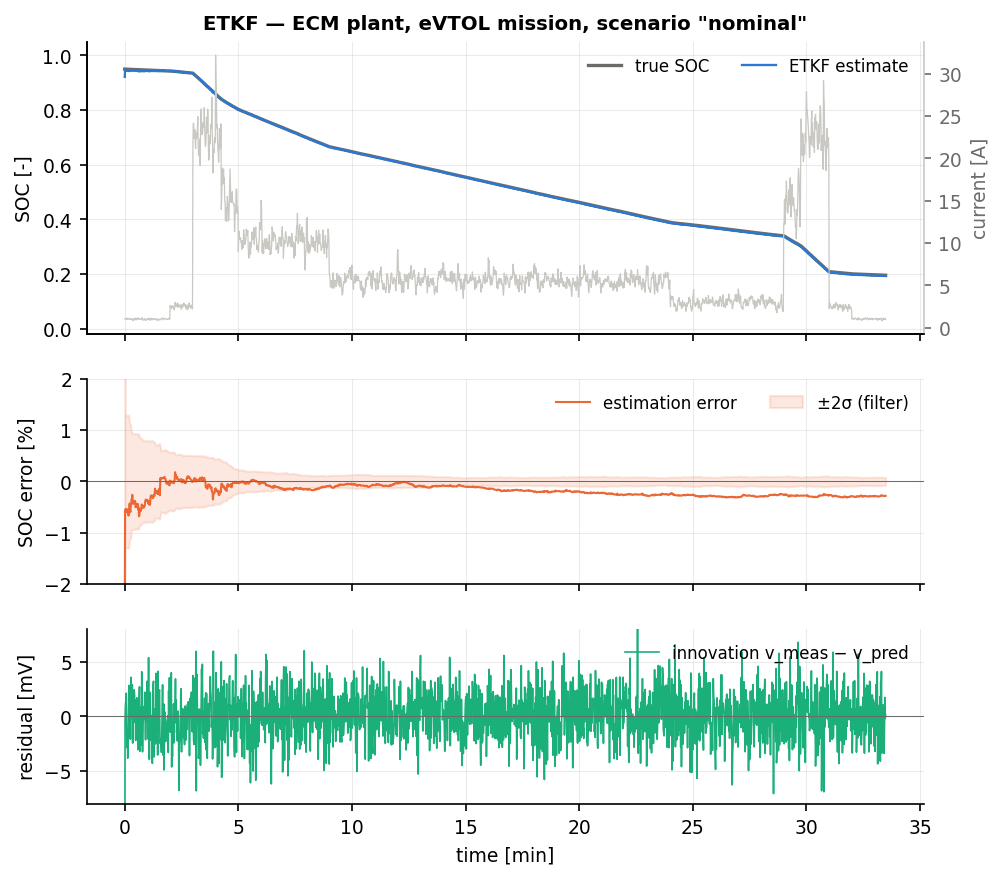
\includegraphics[width=\textwidth]{figures/cell_ETKF_nominal.png}
\caption{ETKF on the nominal eVTOL mission: true and estimated SOC (top), estimation error with the
$\pm2\sigma$ band from the ensemble covariance (middle), voltage residual (bottom).}
\end{figure}
\begin{figure}[H]\centering
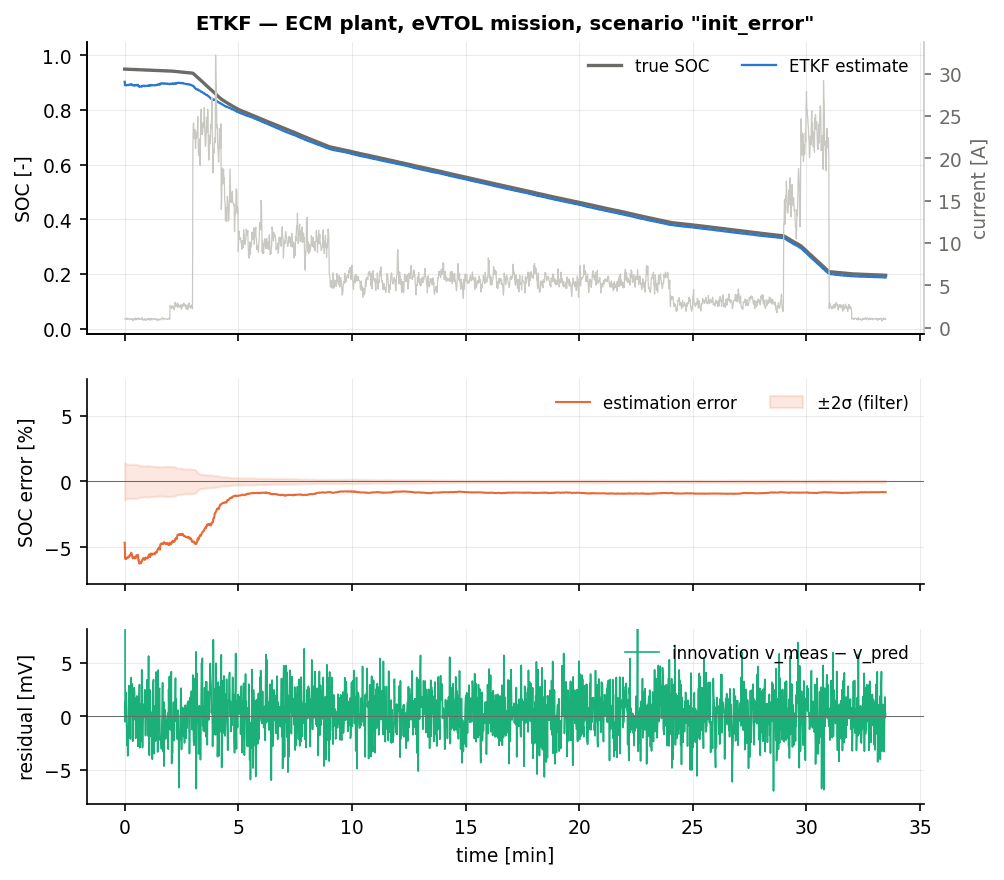
\includegraphics[width=\textwidth]{figures/cell_ETKF_init_error.png}
\caption{ETKF with a \SI{35}{\percent} initial SOC error.  The deterministic transform removes most
of the offset immediately; the remainder is limited by the \num{24}-member sampling error of
$\bm{X}^f$ and is worked off at the rate the inflation permits.}
\end{figure}
\begin{figure}[H]\centering
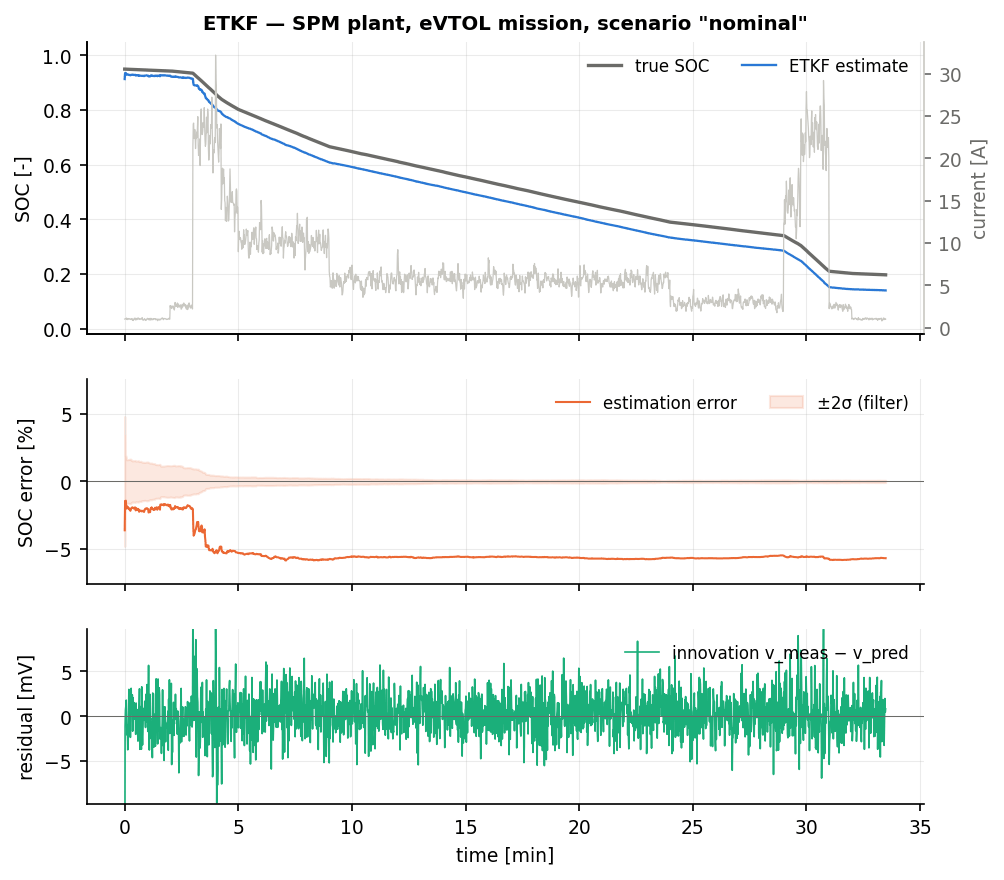
\includegraphics[width=\textwidth]{figures/cellspm_ETKF_nominal.png}
\caption{ETKF on the electrochemical (SPM) plant, nominal mission: \SI{3.82}{\percent}, i.e.\ no
better than the EKF's \SI{3.73}{\percent}.  A deterministic analysis reproduces the Kalman answer
faithfully --- including its bias when the model is wrong.}
\end{figure}

\paragraph{ECM plant.}  On \code{nominal} the ETKF reaches $\mathrm{RMSE} = \SI{0.38}{\percent}$,
$\mathrm{RMSE}_{\mathrm{ss}} = \SI{0.43}{\percent}$, maximum error \SI{3.25}{\percent}, immediate
convergence and a voltage residual of \SI{0.83}{\milli\volt}.  That is slightly \emph{behind} the
stochastic EnKF (\SI{0.27}{\percent}) with half as many members (24 against 50), and the weakest
nominal figure of this family.  The square-root idea is not failing here; the ensemble is simply
smaller, and at $N = 24$ the sampling error of $\bm{X}^f$ costs more than the perturbed
observations do at $N = 50$.

The picture reverses wherever a \emph{persistent} error has to be tracked rather than a random one:
\begin{itemize}[leftmargin=2em]
  \item \code{param\_mismatch}: \SI{0.78}{\percent}, the best result of any estimator in this family
        and a factor \num{1.7} better than the EKF's \SI{1.36}{\percent} (EnKF \SI{3.58}{\percent},
        GSF \SI{2.20}{\percent}).  The deterministic transform contracts the ensemble only in the
        single direction the voltage constrains --- with $n_y = 1$ the matrix $(\bm{Y}^f)^\T\mR\inv\bm{Y}^f$
        is rank one --- and leaves the orthogonal complement inflated by $\sqrt\rho$, which is
        exactly the freedom a mis-parameterised model needs.
  \item \code{cold} \SI{0.71}{\percent} against the EnKF's \SI{1.07}{\percent}, \code{noise\_step}
        \SI{1.72}{\percent} against \SI{1.99}{\percent}, \code{preisach} \SI{0.78}{\percent} against
        \SI{1.00}{\percent} --- and \code{preisach} is the best of the two ensemble filters.
  \item \code{combined} converges in \SI{85}{\second}, by far the fastest of the ensemble pair
        (EnKF \SI{502}{\second}), although its steady-state error there (\SI{4.81}{\percent}) ends
        up worse than the EnKF's \SI{3.75}{\percent}: the deterministic analysis locks on quickly,
        and then has less stochastic freedom to keep adapting once the capacity error starts to
        dominate.
\end{itemize}
Its two weak ECM results are \code{aged\_cell} (\SI{4.61}{\percent}, the worst of the family ---
with $\rho = 1.001$ the ensemble is tighter than the EnKF's, so a persistent capacity error is
absorbed more slowly) and \code{sensor\_dropout} (\SI{1.08}{\percent} against \SI{0.46}{\percent}
for the EKF and \SI{0.33}{\percent} for the EnKF).  During \SI{15}{\second} of frozen voltage the
innovation is a constant non-zero number; the deterministic transform contracts the ensemble around
it every step with no stochastic dithering to slow the collapse, so the filter becomes confidently
wrong.  The stochastic EnKF is accidentally protected by its own perturbations.  An innovation-based
dropout detector would remove this weakness entirely.  Nothing diverges on the ECM plant.

\paragraph{SPM plant.}  This is the one estimator in the family that gains essentially nothing from
the electrochemical plant: \SI{3.82}{\percent} on \code{nominal} against the EKF's
\SI{3.73}{\percent}, \SI{5.40}{\percent} on \code{current\_bias} against \SI{5.69}{\percent},
\SI{9.42}{\percent} on \code{cold} against \SI{7.35}{\percent} (and never converging), and SPM
\code{init\_error} never converging either (\SI{6.72}{\percent}).  The reason is precisely the
property the chapter has been advertising.  The ensemble transform is constructed to reproduce the
Kalman analysis covariance \emph{exactly}, with no Monte-Carlo error --- so when the model is right
it is efficient, and when the model is wrong it reproduces the Kalman \emph{bias} just as exactly.
Its members are not free to wander: after every analysis they are pinned to $\bar{\vx}^f + \bm{X}^f
(\bar{\bm w}^a + \mW^a_{:,i})$, a deterministic contraction of the forecast spread, so there is no
mechanism analogous to the particle filters' roughening or the stochastic EnKF's perturbed forecast
to keep the $(\soc,v_2)$ direction open.  The structured \SI{4}{\milli\volt} residual therefore goes
where the linearised gain sends it --- into SOC.  Multiplicative inflation cannot fix this: $\rho$
re-opens \emph{all} directions isotropically in ensemble space and the sweep above shows what larger
values cost elsewhere.

There is one striking exception, and it confirms the diagnosis: SPM \code{outliers} gives
\SI{0.34}{\percent}, the best result of any estimator on any SPM scenario in this family.  A
\SI{5}{\percent} rate of \SI{50}{\milli\volt} outliers keeps producing innovations far outside
$\mR$, which keeps $(\bm{Y}^f)^\T\mR\inv\bm{Y}^f$ small relative to $(N-1)\mI/\rho$ and so keeps the
transform close to the identity; the ensemble stays wide, the $(\soc,v_2)$ direction stays open, and
the SOC estimate stops absorbing the model residual.  The ETKF is accidentally rescued by noise it
was never designed to handle --- which is a precise way of saying that what it needs on a
mismatched plant is a wider effective prior, not a better square root.

\section{Summary}
The ETKF replaces the stochastic EnKF's perturbed observations by a deterministic transform of the
forecast perturbations, computed in the $N$-dimensional ensemble space from the symmetric square
root of $[(N-1)\mI/\rho + (\bm{Y}^f)^\T\mR\inv\bm{Y}^f]^{-1}$.  The symmetric root is the only choice
that preserves the analysis mean and it minimises the displacement of the ensemble; the
eigen-decomposition it needs is a thirty-line cyclic Jacobi kernel.  At $N=24$ it is the smallest
sampling-based filter in this family (\SI{5.3}{\kilo\byte}, \SI{10.6}{\micro\second}/step), it is
bit-reproducible, and on the ECM plant it delivers the best \code{param\_mismatch} in the family
(\SI{0.78}{\percent} against the EKF's \SI{1.36}{\percent}) and the fastest \code{combined}
convergence of the ensemble pair.  Its caveats are the inflation rate, which must be interpreted per
assimilation cycle and therefore be small at \SI{10}{\hertz}; its over-confidence during a
stuck-sensor fault; and --- the important one --- that an exact reproduction of the Kalman analysis
is an exact reproduction of the Kalman bias: on the electrochemical plant it is the only member of
this family that does no better than the EKF.
